


\begin{frame}{Local Input Space Histograms \sof{1}{3}}

\vspace{1.5em}
\justifying
Prototype-based clustering methods like the {\bf growing neural gas} (GNG) can
suffer from a lack of detail in their input space representation. To amend their
descriptive power we introduced the novel concept of {\bf local input space 
histograms} (LISH) that capture statistical information on the input space lying
between neighboring prototypes~\cite{Kerdels2014a}.

\vspace{1.5em}

\twocol{0.41}{
\justifying
In a regular GNG neighboring prototypes are connected by an edge. We added a 
small histogram to each edge to {\bf capture information on the positions of 
input samples} relative to the respective best and second best matching 
prototypes. 

}{0.5}{
\vspace{-2em}
\begin{figure}
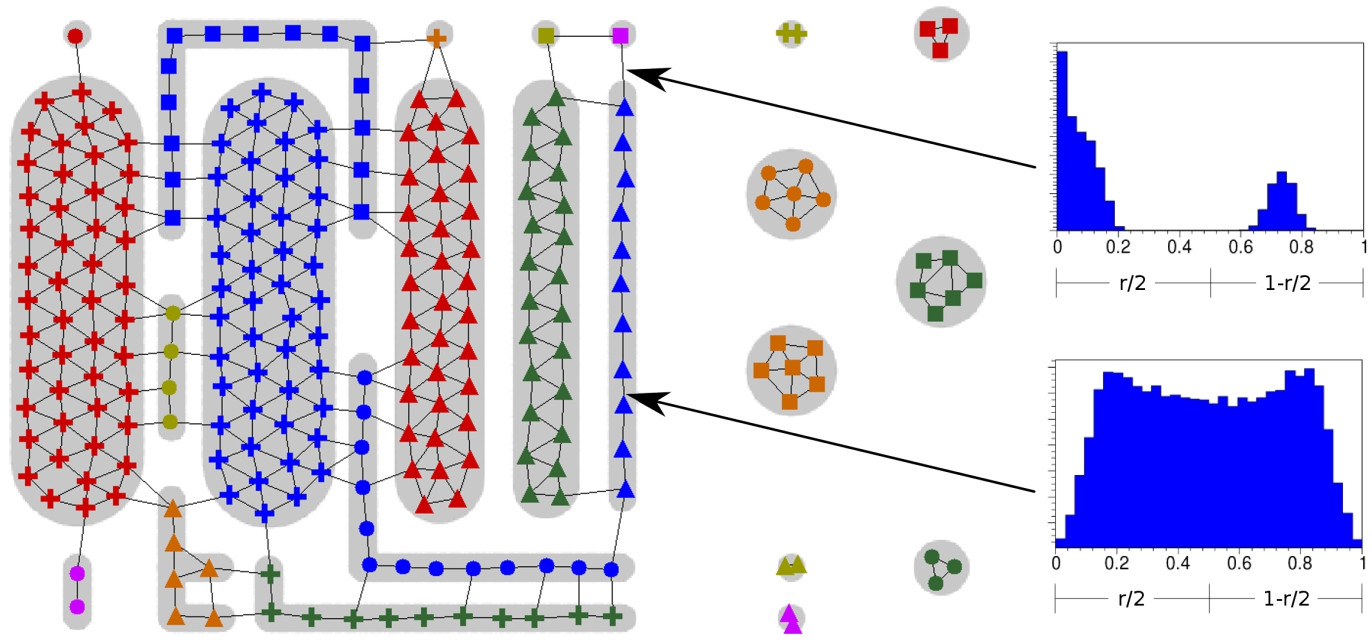
\includegraphics[width=\linewidth]{lish/lish.jpg}

\vspace{-1em}
\caption{\justifying\scriptsize Clustering of an inhomogeneous input space (gray areas) 
with a GNG network of 250 units resulting in 23 clusters (marked by shapes and 
colors of the units). Histograms of two edges are shown on the 
right~\cite{Kerdels2014a}.}
\end{figure}
}

\vspace{1em}
We were able to demonstrate that this additional information can be utilized to,
e.g., {\bf improve clustering} results for challenging, inhomogeneous input 
spaces.

\begin{center}
\rule{2cm}{0.4pt}\\[0.5em]
\end{center}

\fc{Kerdels2014a}{publications/2014-01/2014-01}

\end{frame}



\begin{frame}{Local Input Space Histograms \sof{2}{3}}

\twocol{0.4}{
\vspace{-3em}
\begin{figure}
\hspace{-1.5em}
\adjincludegraphics[width=0.8\linewidth,valign=t]{lish/force-based.jpg}
\vspace{-0.5em}
\caption{\justifying\scriptsize Force-based graph drawing of an image clustering based on
color performed by a LISH enhanced GNG~\cite{Kerdels2015}.}
\adjincludegraphics[width=1.\linewidth,valign=b]{lish/hierarchical.jpg}
\vspace{-1.5em}
\caption{\justifying\scriptsize Hierarchical image clustering based on color performed by 
a LISH enhanced GNG~\cite{Kerdels2015}.}
\end{figure}
}{0.55}{
\justifying

\vspace{1em}
In a follow-up work~\cite{Kerdels2015} we investigate the utility of LISH 
enhanced GNGs for {\bf analysing and clustering high-dimensional data}. Our 
results demonstrate, that the additional information gained about the input 
space structure can be used to enable and improve visualization and hierarchical
clustering. 

\vspace{3.5em}
Furthermore, we show that contrary to common view the {\bf Minkowski distance 
with \(p > 1\) can be a meaningful distance measure} for high-dimensional data.

}

\vspace{-1em}

\begin{center}
\rule{2cm}{0.4pt}\\[0.5em]
\end{center}

\fc{Kerdels2015}{publications/2015-02/2015-02}\\[1em]
\fc{Kerdels2015c}{publications/2015-03/2015-03}\cover

\end{frame}


\begin{frame}{Local Input Space Histograms \sof{3}{3}}

\vspace{1.5em}
\justifying
Further investigation of the LISH concept~\cite{Kerdels2016b} showed that 
information gathered by the LISH can be utilized to form a {\bf relaxed one-hot 
encoding} as the output of a GNG. Processing this output with a second stage GNG
demonstrates that the encoding may serve as a meaningful {\bf sparse 
representation of high-dimensional input spaces}.

\vspace{-0.5em}
\twocol{0.45}{
\begin{figure}
\adjincludegraphics[width=0.7\linewidth,valign=b]{lish/relaxedonehot.jpg}
\caption{\justifying\scriptsize Example of a GNG~\(r\) that processed the relaxed one-hot 
encoded output of a GNG~\(h\) that processed samples from the MNIST database of 
handwritten digits. The shown prototypes reveal the sparse patterns resulting 
from the relaxed one-hot encoding~\cite{Kerdels2016b}.}
\end{figure}
}{0.45}{
\begin{figure}
\adjincludegraphics[width=0.7\linewidth,valign=b]{lish/relaxedonehotvis.jpg}
\caption{\justifying\scriptsize Prototypes of GNG~\(h\) superimposed on the network of 
GNG~\(r\). The shown prototypes correspond to the entry with highest value in 
the respective prototypes of GNG~\(r\)~\cite{Kerdels2016b}.}
\end{figure}

}


\vspace{-1em}

\begin{center}
\rule{2cm}{0.4pt}\\[0.5em]
\end{center}

\fc{Kerdels2016b}{publications/2016-02/2016-02}

\end{frame}


